%TODO: Rellegir sencer
\chapter{Introducció}
\label{sec:introduccio}

En aquest capítol es posa el projecte en el context dels diferents camps d'estudi que aquest abarca: El \emph{Business Process Management} i el \emph{Natural Language Processing}. A continuació, es fa una definició formal del problema que el projecte resol.

\section{Contextualització}
\label{sec:introduccio-contextualitzacio}

Aquesta secció conté una contextualització de l'àmbit d'estudi del projecte. En els següents subapartats es fa referència als camps d'estudi que tenen a veure amb aquest 

\subsection{Business Process Management}
\label{sec:introduccio-bpm}
En el món corporatiu, a l'hora de descriure com opera una empresa se sol parlar en termes de processos de negoci (\emph{business process}). Un procés de negoci es pot definir, de forma abstracta, com una col·lecció de tasques descrites de forma estructurada i que permeten produir un producte o servei concret. En altres paraules, un procés és la descripció de com es duu a terme una certa operació en una empresa, indicant com es mou la informació a través dels diferents agents implicats i quines tasques es realitzen a cada pas.

És en aquest àmbit que apareix el camp del \emph{Business Process Management} (BPM). El BPM engloba l'estudi i modificació d'aquests processos amb l'enfoc específic de millorar-los optimitzant com, i en quin ordre, es porten a terme les tasques que descriu.

Moltes empreses fan servir BPM tant per documentar com per millorar l'eficiència dels seus processos de negoci, i com a resultat d'això, mantenen grans repositoris d'informació amb aquests processos. És vital, doncs, mantenir aquesta informació actualitzada i coherent, i és en aquest problema on neix la motivació per aquest treball.

\subsection{Natural Language Processing}
El \emph{Natural Language Processing} (NLP) és un camp en la informàtica que tracta les interaccions entre els ordinadors i el llenguatge natural dels humans. El NLP tracta diversos tipus de problemes a diferents nivells d'abstracció, des dels més purament linguistics com l'anàlisi morfosintàctic d'oracions o determinar la categoria gramatical d'una paraula (\emph{POS-tagging}) fins a la creació de resums automàtica de notícies d'un diari.

Aquells problemes que tenen a veure amb, no només reconèixer i dividir el text sinó que també pretenen entendre el contingut i derivar-ne informació semàntica cauen en el camp del \emph{Natural Language Understanding} (NLU). L'objectiu del NLU és construir representacions semàntiques completes dels textos, de forma que siguin processables, i.e. comprensibles, per a una màquina. Es tracta, doncs, d'un problema IA-complert \cite[][secció 1]{ai_completeness}, ja que els textos estan escrits per a lectors humans i pressuposen sentit comú i coneixements del món: Coses molt difícils d'incloure en un programa.


\subsection{Descripcions textuals i models de processos}
\label{sec:introduccio-bpm-descripcio}
És evident la necessitat de representar d'alguna manera els processos de negoci per tal que els actors implicats puguin entendre'ls així com perquè els encarregats del \emph{business process management} puguin millorar-los.

La primera forma de representar processos que es tractarà en aquest treball, i també la més evident, és la textual. Consiteix en descriure el procés en un document fent servir llenguatge natural. La figura \ref{fig:example_text} mostra un exemple de representació textual d'un procés. Tot i generalment ser la més senzilla d'interpretar \cite{text_with_bpmn} per les persones implicades en el procés, el fet que es tracti d'informació no estructurada i la ambiguitat inherent al llenguatge natural dificulten molt el tractament d'aquests processos des de l'enfoc del BPM. És per això que apareix el \emph{business process model and notation} (BPMN). 

El BPMN és un estàndard de representació gràfica de processos de negoci creat per la \emph{Business Process Management Initiative} (BPMI)\footnote{Actualment l'estàndard de BPMN està mantingut per l'\emph{Object Management Group} (OMG).}. La figura \ref{fig:example_bpmn} mostra un exemple d'aquesta notació. L'apartat \ref{sec:introduccio-bpmn} conté una descripció més detallada del BPMN.

El BPMN ofereix nombrosos avantatges sobre la representació textual: En primer lloc, permet representar de forma molt més inambigua el contingut, tractant-se d'informació estructurada en forma de diagrama. A més, donada la seva estructura es pot tractar molt més fàcilment amb software; permetent aplicar anàlisi formal per a extreure conclusions globals sobre el comportament dels processos. Finalment, existeixen motors d'execució que a partir d'un BPMN controlen l'execució d'un procés a temps real, permetent a més executar automàticament totes les tasques que puguin ser definides per un \emph{script}. Tot això fa que l'ús del BPMN sigui molt valuós per a una empresa que vulgui automatitzar l'anàlisi i execució dels seus processos.

Els avantatges tecnològics del BPMN respecte a la representació textual són evidents. No obstant això, diferents tipus d'\emph{stakeholders} prefereixen diferents tipus de notació perquè els hi resulta més fàcil d'entendre o perquè no coneixen bé el BPMN.

%====================
% EXEMPLE BPMN I TEXT
%====================
\begin{figure}
\centering
\fbox{\begin{minipage}{0.9\textwidth}
\small\emph{{The examination process can be summarised as follows. The process starts
when the female patient is examined by an outpatient physician, who decides
whether she is healthy or needs to undertake an additional examination. In the
former case, the physician fills out the examination form and the patient can
leave. In the latter case, an examination and follow-up treatment order is placed
by the physician who additionally fills out a request form. Beyond information
about the patient, the request form includes details about the examination 
requested and refers to a suitable lab. Furthermore, the outpatient physician
informs the patient about potential risks. If the patient signs an informed consent
and agrees to continue with the procedure, a delegate of the physician
arranges an appointment of the patient with one of the wards. The latter is
then responsible for taking a sample to be analysed in the lab later. Before the
appointment, the required examination and sampling is prepared by a nurse of
the ward based on the information provided by the outpatient section. Then, a
ward physician takes the sample requested. He further sends it to the lab indicated
in the request form and conducts the follow-up treatment of the patient.
After receiving the sample, a physician of the lab validates its state and decides
whether the sample can be used for analysis or whether it is contaminated and
a new sample is required. After the analysis is performed by a medical technical
assistant of the lab, a lab physician validates the results. Finally, a physician
from the outpatient department makes the diagnosis and prescribes the therapy
for the patient.}}
    \end{minipage}}
    \caption{Exemple de text que descriu un procés de negoci.}
    \label{fig:example_text}
\end{figure}


\begin{figure}
    \begin{center}
        \makebox[\textwidth]{\includegraphics[width=\textwidth]{figures/UlmHospital.png}}
    \end{center}
    %\includegraphics[width=0.9\paperwidth]{UlmHospital.png}
    \caption{Exemple de model BPMN corresponent al text de la figura \ref{fig:example_text}}
    \label{fig:example_bpmn}
\end{figure}
%====================

\subsubsection{Representació dual}
Com que no hi ha un clar vencedor entre la representació textual i la notació BPMN a l'hora de representar processos, moltes vegades s'opta per mantenir el procés documentat d'ambdues maneres. Tenint en compte que en una empresa gran s'estan documentant centenars d'aquests processos, mantinguts per diversos grups de persones i utilitzant diferents eines d'edició és molt probable que tard o d'hora es produeixin inconsistències entre la descripció textual i el model BPMN que representen el mateix procés. Aquestes incoherències són una font de problemes en el procés de producció de l'empresa en qüestió, i solucionar-los manualment requereix una gran inversió en temps i diners.

Donat aquest problema, és evident el gran avantatge d'automatitzar la tasca de comparar el model BPMN amb la corresponent descripció textual, però la dificultat per tractar amb textos no estructurats fa que aquest sigui un terreny molt inexplorat. 


\subsection{La notació BPMN}


En els apartats anteriors s'ha parlat de la notació BPMN. La funció de BPMN és modelar processos de negoci (Veure apartat \ref{sec:introduccio-bpm-descripcio}) i és un estàndard ampliament reconegut i utilitzat per moltes empreses. A nivell d'implementació, està definit com un subonjunt (schema) de XML. L'especificació també descriu una notació visual que s'utilitza per editar i visualitzar els models de procés. En aquesta secció es fa només una breu explicació de la notació BPMN. No obstant, l'especificació d'aquest llenguatge és molt àmplia i, per tant, no es preté donar una explicació exhaustiva. A \cite{bpmn_spec} se'n pot consultar una especificació completa.

El més important de la notació BPMN respecte altres alternatives és que defineix una semàntica d'execució. És a dir, donat un model BPMN, l'execució d'aquest es pot simular de manera automàtica i inambigua. Això permet que les eines de BPM que l'utilitzen puguin coordinar i fins i tot executar algunes parts del procés que defineixen.

En els següents apartats es defineix cadascun dels elements que formen part d'un model BPMN.

\subsubsection{Tasques}

El primer element, i central als processos de negoci són les tasques. Una tasca és una acció que s'ha de realitar en algun punt en l'execució d'un procés de negoci. Les tasques es representen amb un rectangle amb un text. El text ha de contenir simplement el nom de la tasca. Altra informació com el responsable de realitzar-la, o execució sota una condició, s'ha d'indicar mitjançant altres construccions. La figura \ref{fig:task-example} mostra un exemple d'una tasca. 

\begin{figure}[!hbt]
    \centering
    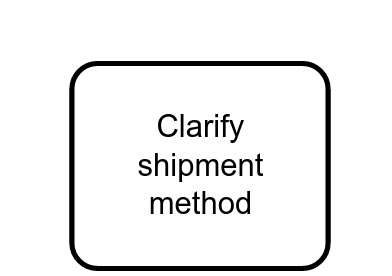
\includegraphics[width=0.3\textwidth]{figures/bpmn-task.png}
    \caption{Una tasca}
    \label{fig:task-example}
\end{figure}

La granularitat de les tasques depèn de l'àmbit de cada problema. En alguns casos caldrà considerar les tasques a un nivell més baix i en altres casos una tasca pot representar diverses hores. La granularitat correcta per a un procés concret és la més gran possible, sempre i quan les tasques segueixin sent atòmiques\footnote{En altres paraules, no es pot indicar lògica en mig d'una tasca, però no té sentit indicar tots i cadascun dels passos d'una tasca si s'han de realitzar sequencialment i sense interrupcions.}. Per exemple, suposem que el cas d'un procés d'un hospital per a determinar si un malalt pateix una certa malaltia. En aquest procés hi podriem trobar tasques com ``Examinar el pacient'' o ``Analitzar les mostres''. Tot i això, en un procés del mateix hospital on s'està parlant de com analitzar els símptomes d'un pacient durant l'examinació, la granularitat de la tasca ``Examinar Pacient'' és massa gran.

\subsubsection{Sequence Flows}

El sequence flow és l'element bàsic per indicar el control de flux entre les tasques. Un sequence flow connecta tasques, events i gateways entre ells. És l'equivalent a una aresta en un graf dirigit i es representa, similarment, amb una fletxa (Figura \ref{fig:sequenceflow-example}). Degut a aquesta similaritat, a la literatura s'utilitza moltes vegades vocabulari similar al dels grafs, anomenant-los arestes o arcs.

\begin{figure}[!hbt]
    \centering
    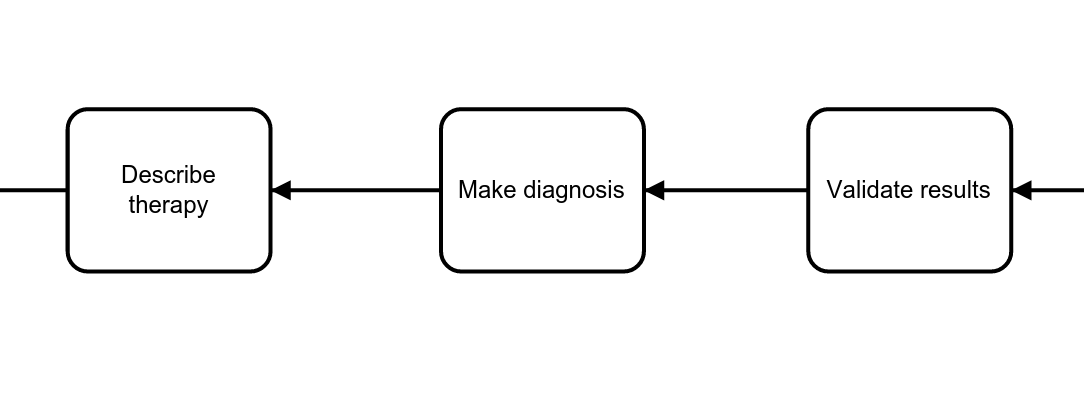
\includegraphics[width=0.8\textwidth]{figures/bpmn-sequenceflows.png}
    \caption{Diferents tasques unides per sequence flows.}
    \label{fig:sequenceflow-example}
\end{figure}


Un sequence flow indica una dependència entre dues tasques. Si la tasca $A$ i la tasca $B$ estan connectades per un sequence flow, la tasca $A$ s'ha de realitzar estrictament abans que $B$.

\subsubsection{Events}

Els events serveixen per modelar successos que poden ocórrer durant l'execució d'un procés. Exemples d'events són: ``Es rep una trucada'', ``Acaba l'execució del programa'', ``Cada 10 minuts''. Els events es representen amb un cercle. La figura \ref{fig:event-example} mostra diferents tipus d'events. Els events es poden connectar a altres events, o tasques, mitjançant sequence flows.

\begin{figure}[!hbt]
    \centering
    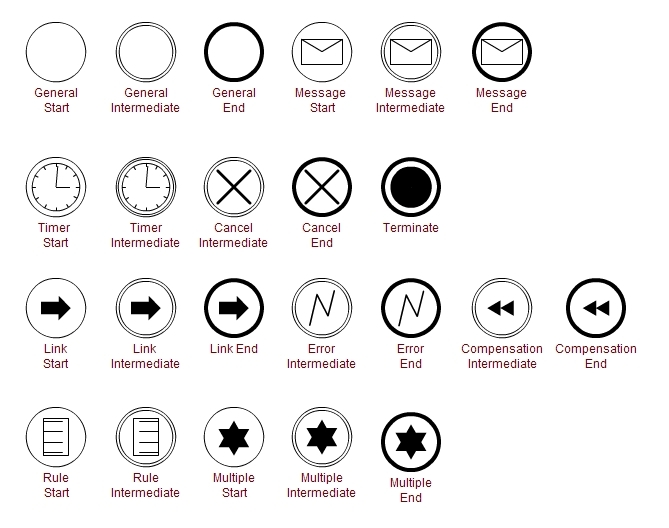
\includegraphics[width=0.7\textwidth]{figures/bpmn-events.jpg}
    \caption{Diferents tipus d'events.}
    \label{fig:event-example}
\end{figure}


Existeixen tres tipus d'events: Start Event, Intermediate Event i End event. Un Start Event és aquell que no té arcs d'entrada. L'execució del model comença sempre en un Start Event. D'altra banda, els End Events sempre acaben un procés, i per tant no poden tenir arcs de sortida. Finalment, els Intermediate Events serveixen per modelar events que puguin ocórrer durant l'execució d'un procés. La tasca que genera un event intermig està connectada a aquest. En un altre punt del model, el mateix event pot tenir un arc de sortida cap una tasca, indicant que quan es produeixi l'event es realitzarà la tasca en questió.

\subsubsection{Gateways}

Les gateway serveixen per indicar el control de flux en un model de procés de negoci. Amb les gateway es poden modelar les construccions típiques dels llenguatges de programació: Execució condicional i Execució en paral·lel. Es representen gràficament amb un quadrat rotat 90 graus. La figura \ref{fig:gateway-example} en mostra els diferents tipus.

\begin{figure}[!hbt]
    \centering
    
\includegraphics[width=0.7\textwidth]{figures/bpmn-gateways.jpg}
    \caption{Diferents tipus de gateway, d'equerra a dreta: Basic, Exclusive, Parallel, Event-Based, Complex i Inclusive.}
    \label{fig:gateway-example}
\end{figure}

Existeixen diferents tipus de gateway, cadascuna amb una semàntica d'execució associada. Les mes típiques són la Exclusive gateway i la Parallel gateway. La exclusiva (Figura \ref{fig:exclusive-gateway-example}), indica una ramificació condicional de l'execució en diversos camins, dels quals s'agafarà un (i només un) en funció de la resposta a una certa pregunta. La paral·lela indica també una ramificació de l'execució, però en aquest cas s'agafen tots els camins i s'executen en paral·lel. Els altres tipus de gateways, menys utilitzats, són la Inclusive Gateway, la Event-Based Gateway i la Complex Gateway, cadascuna amb la seva semàntica particular d'execució. No obstant, és típic a la literatura fer una simplificació i considerar només gateway de tipus paral·lel i exclusiu, ja que les altres es poden modelar a partir d'aquestes dues.

\subsubsection{Pools i swimlanes}

En el text d'una tasca s'hi descriu típicament l'acció, però la frase que la descriu mai acostuma incloure el subjecte. Això és aixi perque aquesta és la tasca de les pools i les swimlanes. Les pools i swimlanes són contenidors dels elements anteriorment mencionats: Tasques, sequence flows, events i gateways. Tant les pools com les gateways tenen un nom, i el nom indica qui, o què, realitza les accions que aquest conté. La figura \ref{fig:pool-swimlane-example} conté un exemple de procés amb una pool i diverses swimlanes.

\begin{figure}[!hbt]
    \centering
    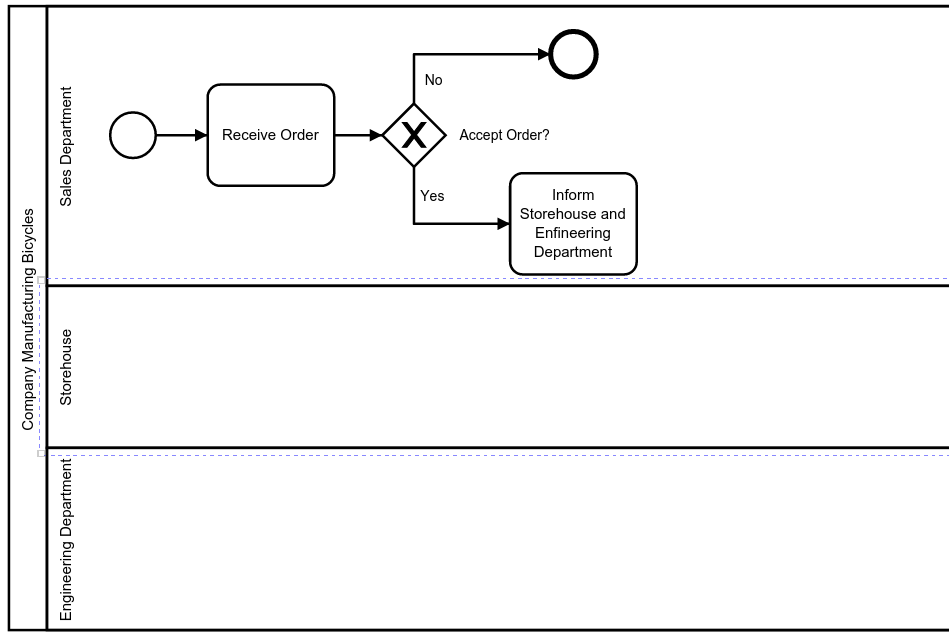
\includegraphics[width=0.8\textwidth]{figures/bpmn-pools.png}
    \caption{Una pool amb tres swimlanes.}
    \label{fig:swimlane-example}
\end{figure}

La diferència entre les pools i les swimlanes és jeràrquica. Una pool pot contenir una o varies swimlanes. A nivell semàntic, la pool sol indicar l'organització que realitza l'acció mentre que la swimlane es refereix a l'actor concret. Per exemple, el director del departament de Recursos Humans, estaria dins la swimlane ``Director'' continguda dins la pool ``Recursos Humans''.

No pot existir cap sequence flow entre elements de diferents pools, però si entre elements de diferents swimlanes. Generalment es diu que cada pool conté un \emph{graf de procés} diferent. Per modelar la comunicació entre elements de diferents pools, s'utilitzen els message flows.

\subsubsection{Message flows}


Els message flow serveixen per indicar la comuniació entre elements de diferents pools. Per exemple, un message flow pot enllaçar una tasca d'una pool amb un event d'una altra pool, indicant que quan aquella tasca es realitzi, s'activarà l'event en una altra pool. Els message flow es representen com una fletxa discontinua.



\section{Estat de l'art}
En aquesta secció es parla de l'estat de l'art en el problema específic que aquest projecte pretén resoldre. 

\subsection{Business Process Management}

El Business Process Management ha rebut molta atenció durant els darrers anys degut al seu potencial per millorar la productivitat de les empreses. En el camp, trobem principalment dues vessants. La primera, que consisteix en l'ús dels models de processos com un suport a la presa de decisions en un entorn corporatiu, permetent als diferents \emph{stakeholders} entendre el problema en qüestió. La segona vessant --més interessant des del punt de vista de la informàtica-, està encarada en l'automatització dels processos per a permetre'n la coordinació automàtica. Aquest darrer camp és conegut pel nom de \emph{Business Process Automation}. Gràcies a les tècniques desenvolupades en BPA, és possible utilitzar eines de software que controlin els processos, executant les tasques automàticament quan això sigui possible, i entregant-les al recurs pertinent, persona o una altra màquina, en cas contrari. Com a producte d'aquesta coordinació automàtica, s'obtenen diverses traces d'execució amb informació detallada que en permeten un anàlisi posterior. Per exemple, si observant les traces es detecta que una tasca concreta és el \emph{bottleneck} del procés, es pot estudiar una solució al problema per millorar la productivitat. Aquest tipus d'anàlisi també juga un paper molt important, no només en l'optimització, sinó també en la detecció d'errors. El conjunt de tècniques d'anàlisi de les traces d'execució rep el nom de \emph{Process Mining}.

Un dels obstacles més grans en el camp del BPM actualment és la falta de consens en la formalització dels processos. Existeixen diversos estàndards per modelar processos de negoci, i no tots estan enfocats en l'automatització dels processos que modelen. Aquesta falta de consens es pot atribuir principalment a dos fets: 

\begin{enumerate}
    \item La complexitat inherent en molts processos de negoci. Ja que moltes vegades les diferents notacions per modelar processos no permeten expressar segons quin tipus de regles complexes.
    \item Els diferents intents en el camp d'estandaritzar una única notació formal per al business process management no han funcionat, creant tot tipus de potencials estàndards diferents.
\end{enumerate}

Tot i que l'enfoc principal en el camp se centra en la millora de productivitat dels processos, diversos estudis destaquen la importància de la verificació formal de processos. La detecció de possibles contradiccions lògiques en un procés de negoci és crucial, sobretot per a permetre'n l'automatització. Si no es verifiquen els processos, poden apareixer errors com \emph{deadlocks} o \emph{livelocks} en l'execució d'un procés. A la literatura, existeixen mesures com la \emph{soundness}\cite{soundness} que pretenen analitzar la correctesa dels models.

Recentment, s'ha començat a investigar l'utilització de tècniques de processat de llenguatge com a eines per al \emph{Business Process Management}. La motivació és, per una banda facilitar el modelat dels processos, i per altra banda permetre l'anàlisi i formalització automàtica de processos no especificats en un llenguatge formal. Han aparegut diversos estudis busquen superar alguns dels obstacles descrits del camp del BPM utilitzant NLP. Alguns d'aquests són:

\begin{itemize}
    \item La conversió automàtica de descripcions textuals, en llenguatge natural, a models de processos \cite{text2bpm}.
    \item La conversió automàtica de models de processos a documents en llenguatge natural.
    \item La comparació automàtica de descripcions textuals i models de processos, camp en el que es troba enmarcat aquest projecte \cite{el_paper}.
\end{itemize}

Un dels desenvolupaments més recents en el processat de llenguatge natural per a BPM és un estudi\cite{nou_paper} on es proposa el concepte de \emph{behavioral space}. L'àmbit de l'estudi se centra en les descripcions textuals de processos, concretament en el fet que les tècniques de NLP no tenen la mateixa capacitat que un humà a l'hora de desambiguar una possible interpretació del significat de les accions d'un procés d'entre totes les possibles. El behavioral space és un enfoc sistemàtic al problema de capturar totes les possibles interpretacions d'una descripció textual d'un procés, en comptes d'haver d'assumir-ne una com a correcta. Els recents resultats obtinguts poden suposar una nova eina molt útil a l'hora de modelar automàticament descrpicions textuals de processos.


\subsection{Natural Language Processing}

En el camp de NLP el focus principal està en interpretar textos cada vegada més complexos, inferint coneixement implícit en el context. Els diferents problemes resolts, en major o menor mesura en NLP són\cite{freeling}:

\begin{itemize}
    \item Separació de textos en frases.
    \item Tokenització, o separació de frases en unitats més simples com paraules o signes de puntuació.
    \item Lematització i Stemming. És a dir, la reducció d'una paraula a la seva arrel, ja sigui utilitzant diccionaris com en el cas de la lemmatització, o aplicant regles simples com en el cas del stemming.
    \item POS-Tagging. El procés de determinar la categoria gramatical de cada paraula\footnote{No només \emph{Determinant}, sinó la categoria completa com \emph{Determinant possessiu}}.
    \item Parsing de constituents, que consisteix a determinar els diferents sintagmes en una frase.
    \item Parsing de dependències, que consisteix a determinar les funcions i relacions entre els elements de la frase. Correspon a l'anàlisi sintàctic.
\end{itemize}

Actualment, l'enfoc en el camp del NLP és sobretot el \emph{Natural Language Understanding} (NLU). El NLU pretén interpretar textos en llenguatge natural per extreure'n informació a alt nivell. Alguns dels problemes encara no resolts en el camp del NLU són:

\begin{description}
    \item[Traducció automàtica intel·ligent]{Consisteix, no només en traduïr textos utilitzant el diccionari, sinó considerar el context de la traducció i coses com frases fetes a l'hora de traduïr.}
    \item[Correcció d'errors]{Consisteix en corregir el text, típicament escrit amb errors, amb possibles errors abans de processar-lo. Un exemple es el pre-tractament de missatges en xarxes socials.}
    \item[Obtenció d'informació]{Similar a un cercador, pero acceptant preguntes formulades en llenguatge natural, i no amb keywords.}
    \item[Extracció d'informació]{A partir d'un text en llenguatge natural, extreure'n les paraules més rellevants i/o fer un resum automàticament.}
\end{description}

El processat de llenguatge natural ha fet servir clàssicament sistemes de regles deterministes com les gramàtiques incontextuals. Més recentment, però, s'han començat a utilitzar tècniques basades en el Machine Learning\cite{nlp_ml} per aprendre a partir de textos reals. Els recents avenços amb les tècniques de machine learning també han permès millores en el processat de llenguatge natural\cite{nlp_dl}. 


\subsection{Comparació de descripcions textuals i models formals de processos}
El problema que tracta aquest projecte, la comparació de models textuals i models de processos en BPMN, és un camp molt inexplorat. Només hi ha un grup \cite{el_paper} que hagi publicat un article proposant una solució a aquest problema. 

La solució que proposa \cite{el_paper} consisteix, igual que aquest projecte, en combinar el BPM amb tècniques de NLP. L'algorisme (veure figura \ref{fig:el_paper_fig}, a grans trets, és el següent:

\begin{enumerate}
    \item Separar el text en frases i el model en tasques.
    \item Analitzar i simplificar el text del model i de les frases amb una eina de NLP\footnote{Concretament l'eina utilitzada és l'\emph{Stanford Parser} \cite{stanford_parser}}.
    \item Computar una \emph{score} de similaritat entre les parelles frase-tasca.
    \item Trobar una assignació òptima que doni la correspondència entre frases del text i tasques del model.
    \item A partir de la informació computada, trobar les inconsistències entre el model i el text.
\end{enumerate}

\begin{figure}[bth]
    \centering
    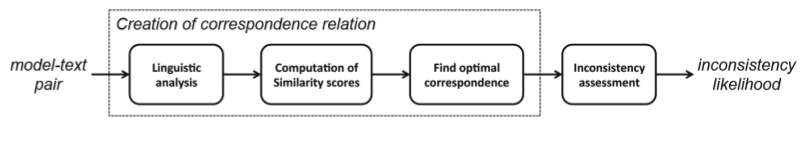
\includegraphics [width=\textwidth]{figures/el_paper_fig.png}
    \caption{Estructura bàsica de la solució proposada en \cite{el_paper}}
    \label{fig:el_paper_fig}
\end{figure}

Centrant-nos en l'apartat d'anàlisi lingüístic, El tractament que es fa a les paraules del text és el següent:

\begin{description}
\item[\textbf{Resolució d'anàfores:}] Els pronoms (\emph{him}, \emph{her}, ...), i alguns determinants (\emph{this}, \emph{that}, ...) del text se substitueixen pel mot al qual fan referència:\\ \emph{him $\rightarrow$ manager}
\item[\textbf{Extracció de clàusules:}] S'eliminen les clàusules secundàries del text, per centrar-se només en les parts de la frase que defineixin una acció del model i eliminar mots que podrien afegir soroll a l'hora de computar similaritats.
\item[\textbf{Sanitització del text:}] S'eliminen les \emph{stopwords}\footnote{Paraules que no aporten significat substancial a la frase, com articles o preposicions.} i les paraules restants se substitueixen per l'arrel del mot:\\ \emph{prepared $\rightarrow$ prepare}
\end{description}



\section{El problema}
\label{sec:introduccio-el_problema}
El problema que es vol resoldre amb aquest projecte es pot resumir amb el següent enunciat: 

\begin{displayquote}
``Donats un model BPMN i una representació textual d'un procés, determinar si corresponen al mateix procés donant una \emph{score} de similaritat i detectar les possibles incoherències que hi pugui haver entre els dos.''
\end{displayquote}

L'objectiu principal del treball és, doncs, la creació de l'algorisme que resol el problema anterior. Més específicament, el treball s'ha dividit en els següents subobjectius:

\begin{enumerate}
    \item Utilitzar tècniques de NLP, fent servir \emph{freeling}\footnote{\emph{Freeling} \cite{freeling} és una eina de software lliure per a \emph{Natural Language Processing} creada pel professor Lluís Padró de la Universitat Politècnica de Catalunya.} des del \emph{Textserver}\footnote{El \emph{Textserver} \cite{textserver} és una plataforma online que proporciona serveis web d'anàlisi linguístic de textos. Fa servir freeling.}, per extreure informació de la descripció textual d'un procés.
    \item Explorar models BPMN i analitzar el seu contingut amb tècniques de NLP i Business Process Management per tal d'extreure'n informació.
    \item Crear una representació homogènia per l'informació extreta del model BPMN i la descripció textual.
    \item Determinar una mètrica de similaritat per comparar la informació extreta.
    \item Establir una noció d'ordre entre elements del text i del model.
    \item Utilitzar un algorisme de satisfacció de restriccions per calcular la correspondència de tasques a frases.
    \item Fer servir tota l'informació obtinguda per tal de detectar possibles incoherències entre el text i el model.
\end{enumerate}
    
\section{Abast}
\label{sec:introduccio-abast}

En aquesta secció es fa una descripció de l'abast d'aquest projecte. L'apartat \ref{sec:introduccio-abast-producte_esperat} parla del producte mínim que es vol aconseguir i possibles ampliacions a aquest. L'apartat \ref{sec:introduccio-abast-obstacles} parla dels obstacles als quals s'enfronta aquest treball.

\subsection{Producte Esperat}
\label{sec:introduccio-abast-producte_esperat}

L'objectiu d'aquest projecte és dissenyar un algorisme que resolgui el problema descrit a la seccio \ref{sec:introduccio-el_problema}. El procés descrit per aquests objectius es pot visualitzar al diagrama de la figura \ref{fig:estructura_projecte}. De les frases i el model se n'extreuen els \emph{UR}\footnote{Abreviació de \emph{Unified Representation}} (Objectius 1, 2 i 3). A continuació es comparen els \emph{UR} d'un cantó amb els de l'altre, per obtenir tant la matriu de similaritat (Objectiu 4) com la de distància (Objectiu 5). Aquestes matrius passen a ser les dades d'entrada d'un algorisme d'optimització per establir l'assignació òptima\footnote{Cal notar que aquesta assignació no ha de ser necessàriament bijectiva.} (Objectiu 6). Finalment s'utilitza la resposta de l'algorisme per determinar on són els punts d'interès i extreure les incoherències que hi puguin haver (Objectiu 7). Per una descripció àmplia de com s'ha plantejat abordar el problema i cadascun d'aquests objectius veure el capítol \ref{sec:enfoc}. 

Com a possibles ampliacions al projecte base, s'han plantejat els següents objectius addicionals:

\begin{enumerate}
    \item Estudiar les possibilitats de reduir el problema a un LAP\footnote{\emph{Linear Assignment Problem} \cite{LAP}}, que té solució en temps polinòmic, per determinar una solució inicial per l'algorisme d'optimització.
    \item Experimentar quina és el millor subconjunt d'informació a extreure eliminant possibles causes de soroll al càlcul de similaritat.
    \item Experimentar amb diverses mètriques de similaritat i fer una comparativa per determinar quina s'escau més al domini del problema.
    \item Investigar i experimentar diferents tipus d'algorismes d'optimització per determinar quin és el més eficient i ofereix millors solucions al problema objectiu.
    \item Estudiar quins tipus d'inconsistències es poden extreure a partir de l'informació calculada.
\end{enumerate}

\begin{figure}
    \centering
    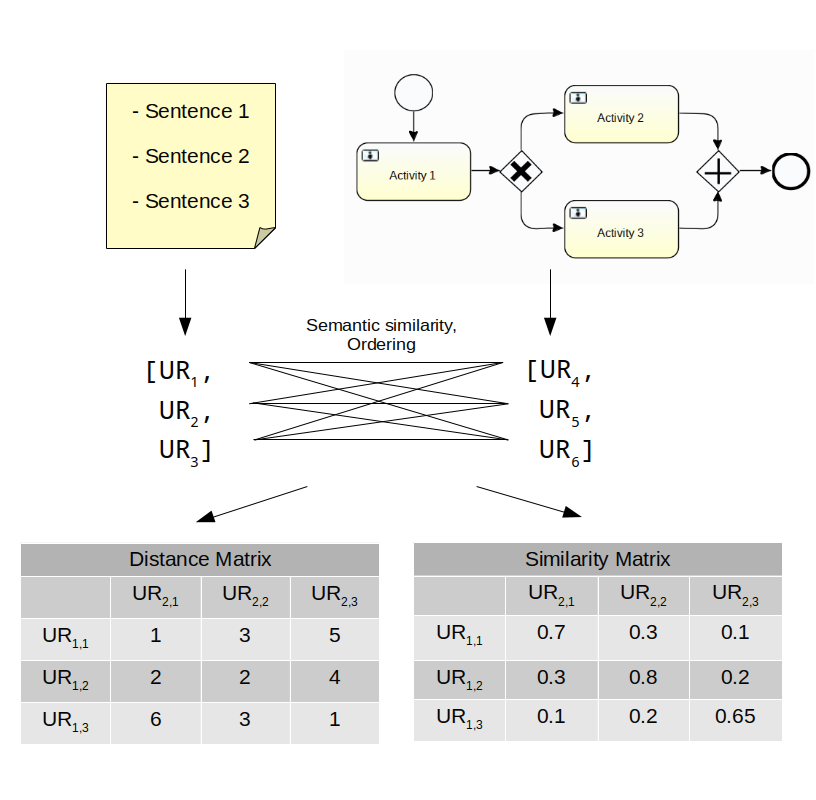
\includegraphics[width=0.8\textwidth]{figures/estructura_projecte.png}
    \caption{Diagrama que representa l'estructura general de l'algorisme.}
    \label{fig:estructura_projecte}
\end{figure}

\subsection{Obstacles}
\label{sec:introduccio-abast-obstacles}
Els obstacles als que s'enfronta aquest projecte provenen de diverses fonts. En alguns casos el problema és tenir massa alternatives i haver d'escollir la millor. En altres casos és la falta d'informació i/o alternatives. D'altres són dificultats tècniques que queden totalment fora de l'abast del projecte. Aquest apartat és un recull de les possibles limitacions i obstacles que han aparegut en plantejar el projecte:

\begin{itemize}
    \item La falta de coneixement del món per part de les eines de NLP utilitzades dificulten la possibilitat de determinar que dues frases  referint al mateix. Aquest problema es pot exemplificar amb les frases: \emph{The patient can leave} (text) i \emph{Release patient} (BPMN). Les dues frases corresponen a la mateixa acció, però l'elecció de paraules del segon implica un coneixement del món de la medicina mitjançant el qual es pot deduïr que el pacient és una persona que ha estat donada d'alta i que per tant els verbs \emph{release} i \emph{leave} s'estan referint a la mateixa acció quan en general no ho fan. 
    \item La falta de dades d'exemple, ja que les empreses no solen compartir la documentació dels seus processos per motius de secret professional. Sense un repositori de dades reals d'exemple és difícil experimentar amb diferents opcions de l'algorisme i avaluar-ne la qualitat. Aquesta falta de dades també dificulta possibles opcions com el machine learning a l'hora de determinar els paràmetres de l'algorisme.
    \item La quantitat d'opcions quant a algorismes d'optimització i mètriques de similaritat fa que quedi fora de l'abast d'aquest projecte provar-los tots i avaluar-ne la qualitat.
    \item Donat que el projecte pretén comparar textos i models BPMN, és difícil avaluar la qualitat de l'algorisme de forma automàtica, ja que per fer-ho caldria resoldre el mateix problema que pretén resoldre aquest.
\end{itemize}



%TODO: El nom me l'he inventat, però cal un nom
\section{El projecte NLP4BPM}

Aquest projecte es troba dins el marc d'un projecte més gran: NLP4BPM\footnote{\emph{Natural Language Processing} for \emph{Business Process Management}}. El projecte NLP4BPM és una iniciativa que pretén combinar els móns del \emph{Business Process Management} i el \emph{Natural Language Processing} amb l'objectiu de la creació d'una eina per assistir en l'automatització de tasques relacionades amb el camp del BPM. El projecte s'ha desenvolupat fins al moment a partir de diversos treballs de final de grau, un d'ells encarregat d'integrar tots els algorismes en una plataforma web que proporcioni una interfície gràfica uniforme per a tot el software. Les diferents parts que s'han implementat amb diversos treballs han estat fins a la data:

\begin{itemize} 
        \item Un traductor de descripcions textuals a models BPMN. Desenvolupat per Dídac Martínez i Arnau Gil.
        \item Un traductor de models BPMN a descripcions textuals. Desenvolupat per Genís Martín.
        \item Una eina que permeti comparar models BPMN i descripcions textuals. Desenvolupada per Josep Sánchez Ferreres. Aquesta eina correspon al projecte d'aquesta memòria.
        \item Una eina que permeti comparar models BPMN entre ells. Desenvolupada per Luis Delicado.
        \item Una eina gràfica que integri (figura \ref{fig:ui}) totes les funcionalitats anteriors en una plataforma web. Desenvolupada per Luis Delicado Alcántara.
\end{itemize}

\begin{figure}[!htb]
    \centering
    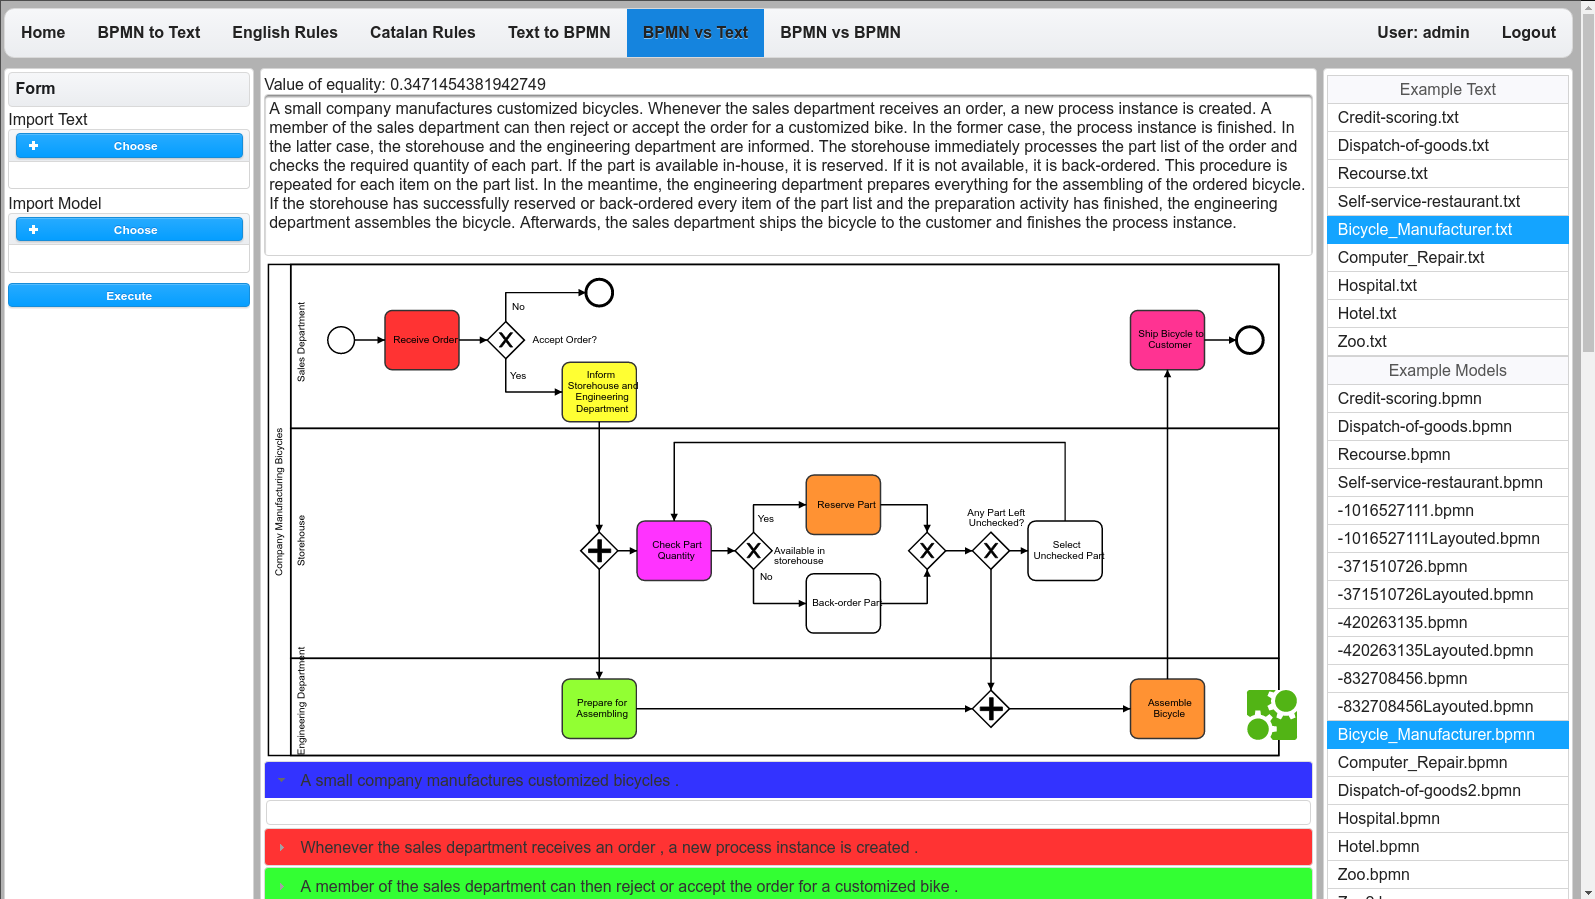
\includegraphics[width=\textwidth]{figures/interficie1.png}
    \caption{Captura de pantalla de la versió final del projecte executant-se a la plataforma web.}
    \label{fig:ui}
\end{figure}

